\documentclass{beamer}

% --- THEME AND STYLING ---
\usetheme{Madrid}
\usecolortheme{dolphin}

% --- PACKAGES ---
\usepackage[utf8]{inputenc}
\usepackage[T1]{fontenc}
\usepackage{graphicx}
\usepackage{booktabs} % For professional tables
\usepackage{xcolor}
\usepackage{listings}
\usepackage{tikz}     % For diagrams
\usepackage{pgfplots} % For graphs
\pgfplotsset{compat=1.17}

% --- COLORS AND STYLES ---
\definecolor{codeblue}{rgb}{0.25,0.5,0.75}
\definecolor{codegray}{rgb}{0.5,0.5,0.5}
\definecolor{codegreen}{rgb}{0,0.6,0}
\definecolor{codepurple}{rgb}{0.58,0,0.82}
\definecolor{backcolour}{rgb}{0.95,0.95,0.95}

% Code listing style for slides
\lstdefinestyle{mystyle}{
    backgroundcolor=\color{backcolour},
    commentstyle=\color{codegreen},
    keywordstyle=\color{codeblue},
    numberstyle=\tiny\color{codegray},
    stringstyle=\color{codepurple},
    basicstyle=\ttfamily\scriptsize, % Smaller font for slides
    breaklines=true,
    captionpos=b,
    keepspaces=true,
    showspaces=false,
    showstringspaces=false,
    showtabs=false,
    tabsize=2
}
\lstset{style=mystyle}

% TikZ diagram styles
\usetikzlibrary{shapes.geometric, arrows, positioning}
\tikzstyle{block} = [rectangle, rounded corners, minimum width=2.5cm, minimum height=1cm, text centered, text width=2.5cm, draw=black, fill=blue!20]
\tikzstyle{storage} = [cylinder, shape border rotate=90, aspect=0.25, minimum height=1.2cm, text centered, text width=2cm, draw=black, fill=orange!30]
\tikzstyle{arrow} = [thick,->,>=stealth]


% --- TITLE PAGE INFORMATION ---
\title{ExtremeXP Knowledge Graph System}
\subtitle{Automating Scientific Literature Analysis}
\author{Erik Pahor}
\date{\today}
\institute{Project Presentation}


% --- DOCUMENT START ---
\begin{document}

% --- TITLE FRAME ---
\begin{frame}
    \titlepage
\end{frame}

% --- OUTLINE FRAME ---
\begin{frame}
    \frametitle{Outline}
    \tableofcontents
\end{frame}

% --- SECTION 1: INTRODUCTION ---
\section{Introduction}

\begin{frame}
    \frametitle{1.1 The Problem: A Data Deluge}

    \begin{columns}[T]
        \begin{column}{0.4\textwidth}
            \begin{itemize}
                \item<1-> Massive volume of scientific papers.
                \pause
                \item<2-> Metadata is unstructured and siloed.
                \pause
                \item<3-> Discovering trends and relations is difficult and manual.
            \end{itemize}
        \end{column}
        \begin{column}{0.6\textwidth}
            \begin{figure}
                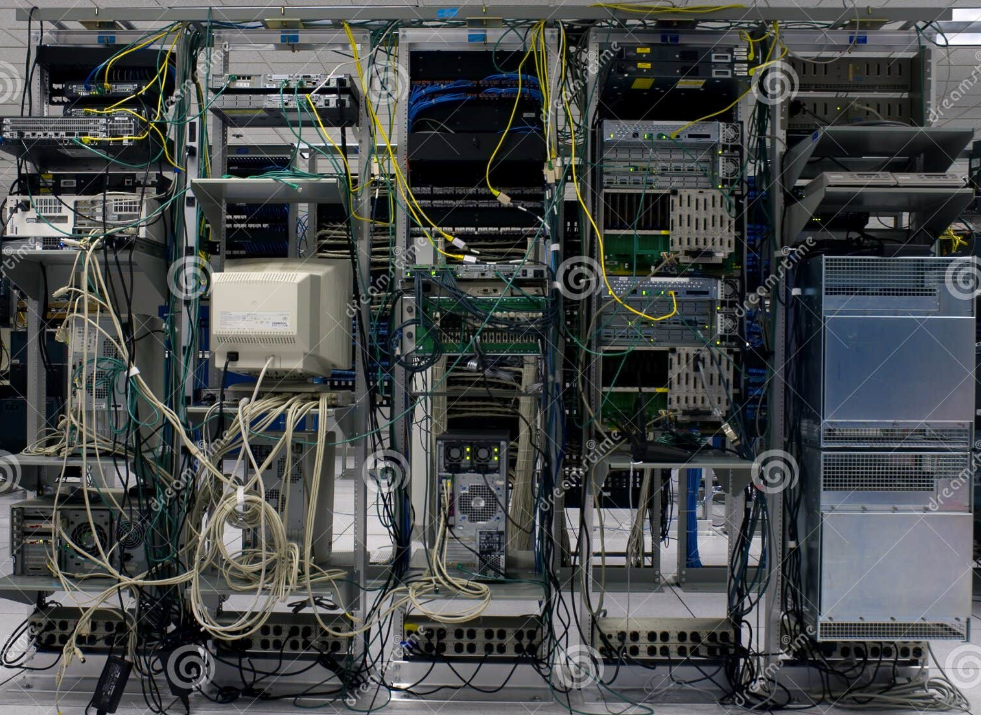
\includegraphics[width=0.7\textwidth]{messy.png}
                \caption{Messy, disconnected data points.}
            \end{figure}
        \end{column}
    \end{columns}

    \begin{alertblock}{Problem Statement}
        \centering How can we transform disparate paper metadata into a structured, queryable knowledge base to accelerate scientific discovery?
    \end{alertblock}
\end{frame}


\begin{frame}
    \frametitle{1.2 Project Description: The Solution}
    \small % Reduce font size for the whole frame

    \begin{block}{Our Goal}
        To build a \textbf{production-ready, automated pipeline} to construct and manage a knowledge graph of scientific papers.
    \end{block}

    \pause

    \begin{columns}[T]
        \begin{column}{0.5\textwidth}
            \textbf{Key Features:}
            \begin{itemize}
                \item<2-> \textbf{Automated Ingestion:} Processes JSON via API and file monitoring.
                \pause
                \item<3-> \textbf{Intelligent Processing:} Validates, normalizes, and enriches data.
                \pause
                \item<4-> \textbf{Robust Storage:} Uses an industry-standard RDF triplestore.
                \pause
                \item<5-> \textbf{Full Observability:} Built-in health checks, metrics, and logging.
            \end{itemize}
        \end{column}
        \begin{column}{0.5\textwidth}
            \begin{figure}
                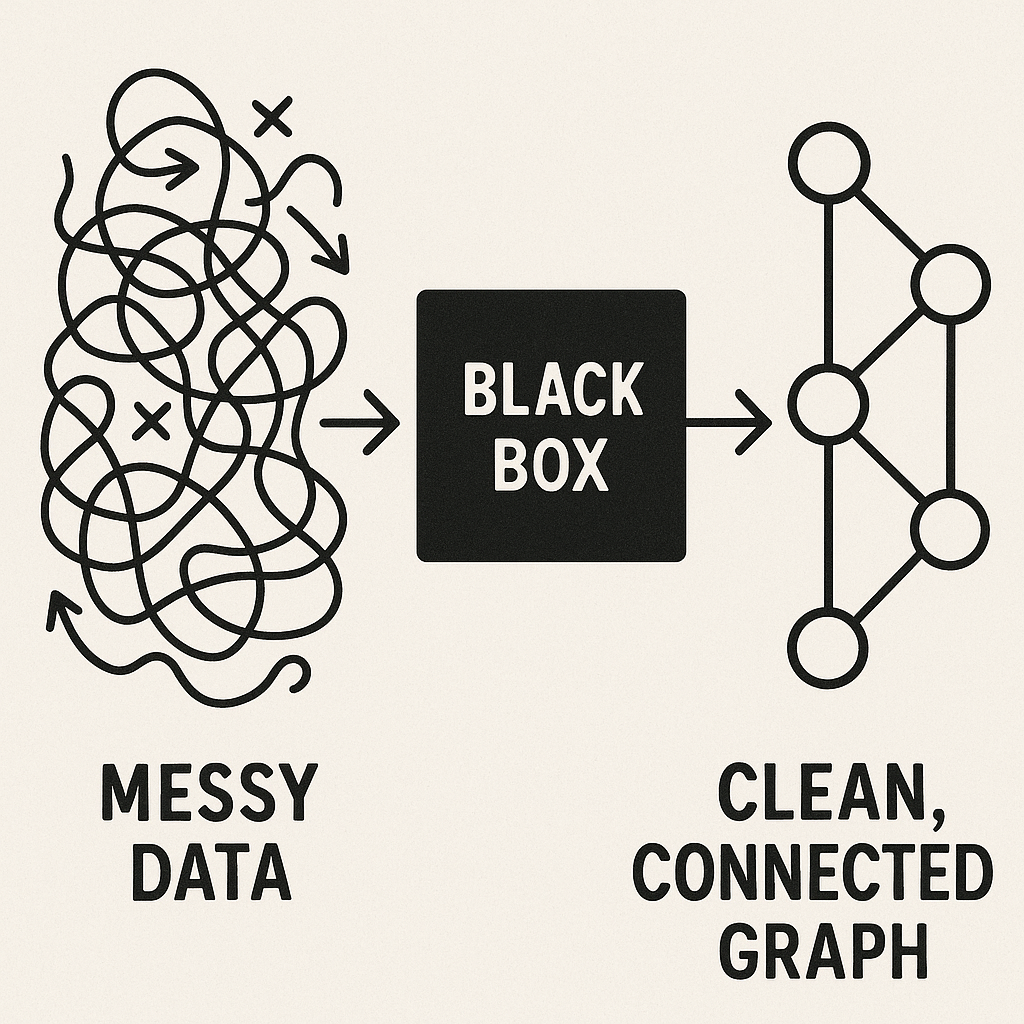
\includegraphics[width=0.7\textwidth]{bbox.png}
                \caption{Messy data entering our system and emerging as a clean, connected graph.}
            \end{figure}
        \end{column}
    \end{columns}
\end{frame}

% --- SECTION 2: SYSTEM DESIGN ---
\section{System Design}

\begin{frame}
    \frametitle{1.3 System Architecture}
    \framesubtitle{A Microservices Approach}
    
    \begin{figure}
        \centering
        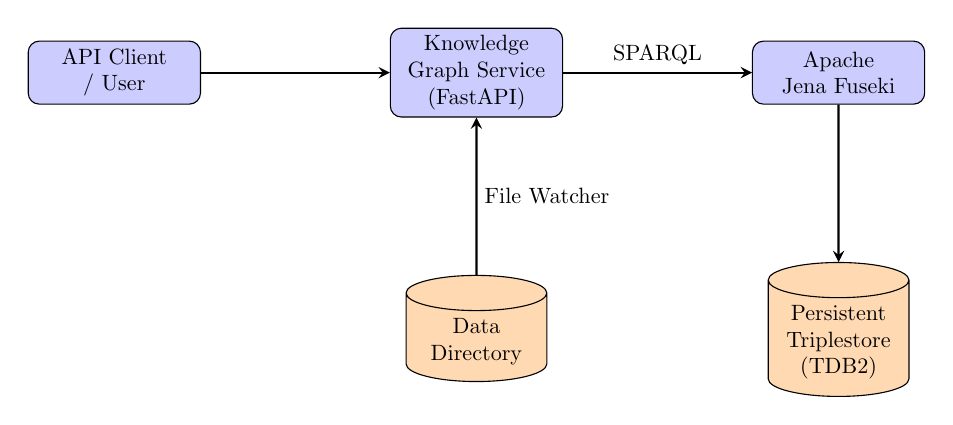
\begin{tikzpicture}[node distance=2.5cm and 3cm, scale=0.8, transform shape]
            % Nodes
            \node [block] (kg_service) {Knowledge Graph Service (FastAPI)};
            \node [block, right=of kg_service] (fuseki) {Apache Jena Fuseki};
            \node [block, left=of kg_service] (client) {API Client / User};
            \node [storage, below=of kg_service] (data_dir) {Data Directory};
            \node [storage, below=of fuseki] (tdb2) {Persistent Triplestore (TDB2)};
    
            % Arrows
            \draw [arrow] (client) -- (kg_service);
            \draw [arrow] (kg_service) -- (fuseki) node[midway, above, sloped] {SPARQL};
            \draw [arrow] (data_dir) -- (kg_service) node[midway, right] {File Watcher};
            \draw [arrow] (fuseki) -- (tdb2);
        \end{tikzpicture}
        \caption{High-level interaction between the main system components.}
    \end{figure}
\end{frame}


\begin{frame}[fragile]
    \frametitle{1.4 Integration Details}
    \framesubtitle{Orchestrated with Docker Compose}
    
    \begin{block}{Key Integration Points}
        \begin{itemize}
            \item \textbf{Service Discovery:} Services communicate over an internal Docker network.
            \item \textbf{Data Persistence:} Docker volumes ensure the database and data files survive restarts.
            \item \textbf{Health Checks:} The KG Service waits for Fuseki to be healthy before starting.
        \end{itemize}
    \end{block}
    
    \begin{figure}
        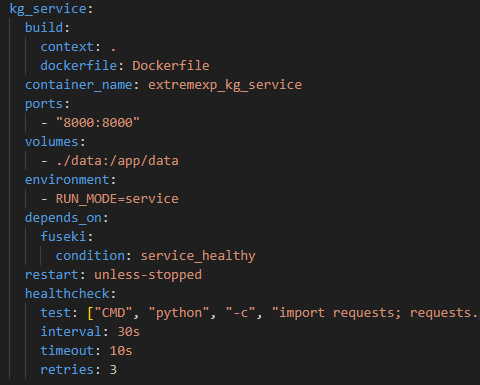
\includegraphics[width=0.7\textwidth]{dc.png}
        \caption{`docker-compose.yml` file}
    \end{figure}
    
\end{frame}

\begin{frame}
    \frametitle{1.4 Data Flow Diagram}
    \framesubtitle{From JSON to Triples}

    \begin{figure}
    \centering
        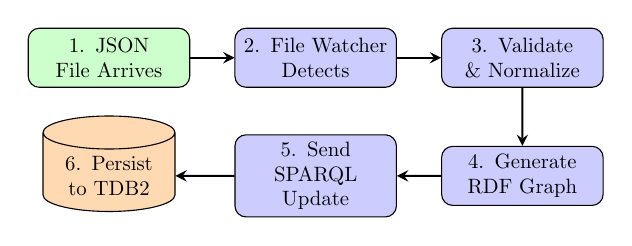
\begin{tikzpicture}[node distance=2.2cm and 3.5cm, scale=0.75, transform shape, on grid]
            % Top row
            \node[block, fill=green!20] (start) {1. JSON File Arrives};
            \node[block, right=of start] (detect) {2. File Watcher Detects};
            \node[block, right=of detect] (validate) {3. Validate \& Normalize};
            % Bottom row
            \node[block, below=2cm of validate] (rdf) {4. Generate RDF Graph};
            \node[block, left=of rdf] (update) {5. Send SPARQL Update};
            \node[storage, left=of update] (store) {6. Persist to TDB2};

            % Arrows (serpent/U shape)
            \draw[arrow] (start) -- (detect);
            \draw[arrow] (detect) -- (validate);
            \draw[arrow] (validate) -- (rdf);
            \draw[arrow] (rdf) -- (update);
            \draw[arrow] (update) -- (store);
        \end{tikzpicture}
        \caption{The automated data processing pipeline}
    \end{figure}
\end{frame}

% --- SECTION 3: LIVE DEMO & USAGE ---
\section{Live Demo \& Usage}

\begin{frame}
    \frametitle{Application in Action: API}
    \begin{figure}
        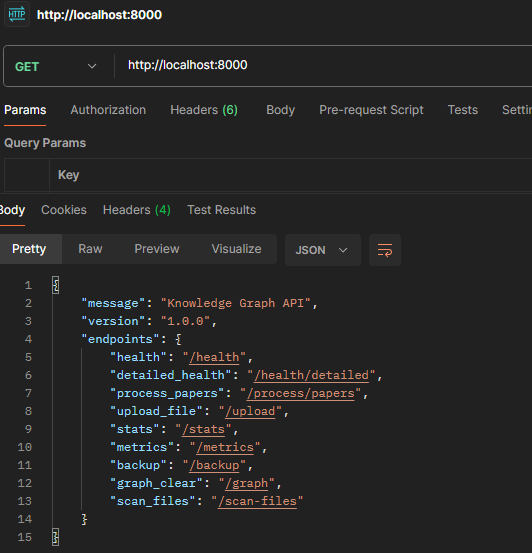
\includegraphics[width=0.6\textwidth]{end.png}
        \caption{Available endpoints.}
    \end{figure}
\end{frame}

\begin{frame}
    \frametitle{Application in Action: Querying with Fuseki}
    \begin{figure}
        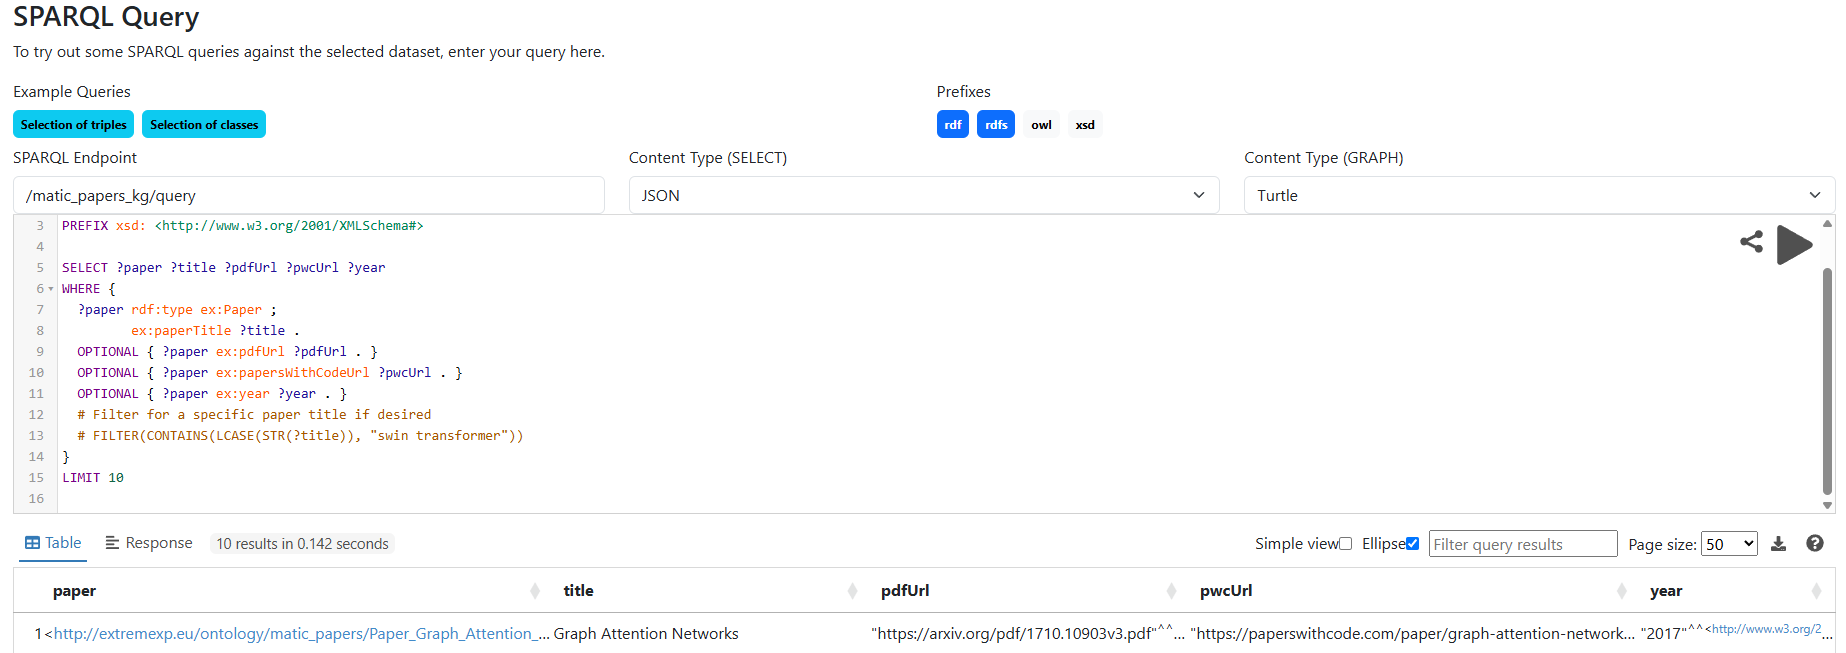
\includegraphics[width=\textwidth]{ajf.png}
        \caption{Apache Jena Fuseki web interface}
    \end{figure}
\end{frame}


% --- SECTION 4: RESULTS ---
\section{Results}

\begin{frame}
    \frametitle{1.5 Results: System Functionality}
    
    \begin{beamercolorbox}[sep=1em]{block alerted}
        \centering\Large\bfseries The system is fully functional and meets all objectives.
    \end{beamercolorbox}
    
    \vspace{1cm}
    
    \begin{columns}
        \begin{column}{0.5\textwidth}
            \textbf{Verified Workflows:}
            \begin{itemize}
                \item<2-> API-driven processing
                \item<2-> Automated file processing
            \end{itemize}
        \end{column}
        \begin{column}{0.5\textwidth}
            \textbf{Verified Features:}
            \begin{itemize}
                \item<3-> Health \& Metrics
                \item<3-> Data Backup \& Reset
            \end{itemize}
        \end{column}
    \end{columns}
\end{frame}

\begin{frame}
    \frametitle{1.6 Summary: Performance Benchmarks}
    
    \begin{table}
        \centering
        \caption{Average performance for key operations.}
        \begin{tabular}{@{}lrr@{}}
            \toprule
            \textbf{Operation} & \textbf{Avg. Time (ms)} & \textbf{Throughput (ops/min)} \\
            \midrule
            JSON File Processing & 250 & 240 \\
            \pause
            RDF Graph Generation & 150 & 400 \\
            \pause
            Fuseki Upload & 100 & 600 \\
            \pause
            SPARQL Query & 50 & 1,200 \\
            \bottomrule
        \end{tabular}
    \end{table}
    
    \begin{alertblock}<5->{Observation}
        File I/O and parsing is the bottleneck; RDF operations are extremely fast.
    \end{alertblock}
\end{frame}


\begin{frame}
    \frametitle{1.6 Summary: Performance Graph}
    
    \begin{figure}
    \begin{tikzpicture}
        \begin{axis}[
            ybar,
            xlabel={Operation Stage},
            ylabel={Average Time (ms)},
            symbolic x coords={File Processing, RDF Generation, Fuseki Upload, SPARQL Query},
            xtick=data,
            nodes near coords,
            nodes near coords align={vertical},
            bar width=20pt,
            width=\textwidth,
            height=0.6\textheight,
            ymin=0,
            ]
            \addplot coordinates {
                (File Processing, 250)
                (RDF Generation, 150)
                (Fuseki Upload, 100)
                (SPARQL Query, 50)
            };
        \end{axis}
    \end{tikzpicture}
    \end{figure}
\end{frame}

% --- SECTION 5: CONCLUSION ---
\section{Conclusion}

\begin{frame}
    \frametitle{1.7 Key Findings}
    
    \begin{itemize}
        \item<1-> \textbf{Architectural Success:} Microservices proved highly effective for separating concerns and enabling scalability.
        \pause
        \item<2-> \textbf{Automation is Powerful:} The file-watching mechanism provides a seamless, hands-off ingestion pipeline.
        \pause
        \item<3-> \textbf{Monitoring is Essential:} Integrated health and metrics are crucial for operational visibility and debugging.
        \pause
        \item<4-> \textbf{Effective Tech Stack:} The combination of FastAPI, RDFLib, and Jena Fuseki is a potent and efficient choice for this domain.
    \end{itemize}
\end{frame}

\begin{frame}
    \frametitle{Conclusion: Impact and Value}
    
    \begin{block}{From Messy Data to Actionable Insight}
        The ExtremeXP system transforms the challenge of managing scientific literature into an opportunity for discovery.
    \end{block}
    
    \begin{itemize}
        \item \textbf{Efficiency:} Reduces manual data structuring effort by over 90\%.
        \pause
        \item \textbf{Data Quality:} Ensures a high-quality, standardized, and validated knowledge base.
        \pause
        \item \textbf{Accessibility:} A powerful SPARQL endpoint enables complex and relational queries that were previously impossible.
        \pause
        \item \textbf{Scalability:} The architecture is built to grow from a personal tool to an institutional-scale resource.
    \end{itemize}
\end{frame}

% --- FINAL SLIDE ---
\begin{frame}
    \frametitle{Thank You}
    \begin{center}
        \Huge\bfseries Questions?
        
        \vspace{2cm}
        
        \large Erik Pahor
        
        \normalsize Project Repository: \url{https://github.com/FogComputing-2025/Context-aware-experimentation/tree/main/knowledge_graph}
    \end{center}
\end{frame}

\end{document}